\documentclass[12pt]{article}
\usepackage[left=1cm, right=1cm, top=2cm,bottom=1.5cm]{geometry} 

\usepackage[parfill]{parskip}
\usepackage[utf8]{inputenc}
\usepackage[T2A]{fontenc}
\usepackage[russian]{babel}
\usepackage{enumitem}
\usepackage[normalem]{ulem}
\usepackage{amsfonts, amsmath, amsthm, amssymb, mathtools,xcolor,accents}
\usepackage{blkarray}

\usepackage{tabularx}
\usepackage{hhline}

\usepackage{accents}
\usepackage{fancyhdr}
\pagestyle{fancy}
\renewcommand{\headrulewidth}{1.5pt}
\renewcommand{\footrulewidth}{1pt}

\usepackage{graphicx}
\usepackage[figurename=Рис.]{caption}
\usepackage{subcaption}
\usepackage{float}

%%Наименование папки откуда забирать изображения
\graphicspath{ {./images/} }

%%Изменение формата для ввода доказательства
\renewcommand{\proofname}{$\square$  \nopunct}
\renewcommand\qedsymbol{$\blacksquare$}

%%Изменение отступа на таблицах
\addto\captionsrussian{%
	\renewcommand{\proofname}{$\square$ \nopunct}%
}
%% Римские цифры
\newcommand{\RN}[1]{%
	\textup{\uppercase\expandafter{\romannumeral#1}}%
}

%% Для удобства записи
\newcommand{\MR}{\mathbb{R}}
\newcommand{\MC}{\mathbb{C}}
\newcommand{\MQ}{\mathbb{Q}}
\newcommand{\MN}{\mathbb{N}}
\newcommand{\MZ}{\mathbb{Z}}
\newcommand{\MTB}{\mathbb{T}}
\newcommand{\MTI}{\mathbb{I}}
\newcommand{\MI}{\mathrm{I}}
\newcommand{\MCI}{\mathcal{I}}
\newcommand{\MJ}{\mathrm{J}}
\newcommand{\MH}{\mathrm{H}}
\newcommand{\MT}{\mathrm{T}}
\newcommand{\MU}{\mathcal{U}}
\newcommand{\MV}{\mathcal{V}}
\newcommand{\MA}{\mathcal{A}}
\newcommand{\MB}{\mathcal{B}}
\newcommand{\MF}{\mathcal{F}}
\newcommand{\ME}{\mathcal{E}}
\newcommand{\MW}{\mathcal{W}}
\newcommand{\ML}{\mathcal{L}}
\newcommand{\MP}{\mathcal{P}}
\newcommand{\VN}{\varnothing}
\newcommand{\VE}{\varepsilon}
\newcommand{\dx}{\, dx}
\newcommand{\dy}{\, dy}
\newcommand{\dz}{\, dz}
\newcommand{\dd}{\, d}


\theoremstyle{definition}
\newtheorem{defn}{Опр:}
\newtheorem{rem}{Rm:}
\newtheorem{prop}{Утв.}
\newtheorem{exrc}{Упр.}
\newtheorem{problem}{Задача}
\newtheorem{lemma}{Лемма}
\newtheorem{theorem}{Теорема}
\newtheorem{corollary}{Следствие}

\newenvironment{cusdefn}[1]
{\renewcommand\thedefn{#1}\defn}
{\enddefn}

\DeclareRobustCommand{\divby}{%
	\mathrel{\text{\vbox{\baselineskip.65ex\lineskiplimit0pt\hbox{.}\hbox{.}\hbox{.}}}}%
}
\DeclareRobustCommand{\ndivby}{\mkern-1mu\not\mathrel{\mkern4.5mu\divby}\mkern1mu}


%Короткий минус
\DeclareMathSymbol{\SMN}{\mathbin}{AMSa}{"39}
%Длинная шапка
\newcommand{\overbar}[1]{\mkern 1.5mu\overline{\mkern-1.5mu#1\mkern-1.5mu}\mkern 1.5mu}
%Функция знака
\DeclareMathOperator{\sgn}{sgn}

%Функция ранга
\DeclareMathOperator{\rk}{\text{rk}}
\DeclareMathOperator{\diam}{\text{diam}}


%Обозначение константы
\DeclareMathOperator{\const}{\text{const}}

\DeclareMathOperator{\codim}{\text{codim}}

\DeclareMathOperator*{\dsum}{\displaystyle\sum}
\newcommand{\ddsum}[2]{\displaystyle\sum\limits_{#1}^{#2}}
\newcommand{\ddssum}[2]{\displaystyle\smashoperator{\sum\limits_{#1}^{#2}}}
\newcommand{\ddlsum}[2]{\displaystyle\smashoperator[l]{\sum\limits_{#1}^{#2}}}
\newcommand{\ddrsum}[2]{\displaystyle\smashoperator[r]{\sum\limits_{#1}^{#2}}}

%Интеграл в большом формате
\DeclareMathOperator{\dint}{\displaystyle\int}
\newcommand{\ddint}[2]{\displaystyle\int\limits_{#1}^{#2}}
\newcommand{\ssum}[1]{\displaystyle \sum\limits_{n=1}^{\infty}{#1}_n}

\newcommand{\smallerrel}[1]{\mathrel{\mathpalette\smallerrelaux{#1}}}
\newcommand{\smallerrelaux}[2]{\raisebox{.1ex}{\scalebox{.75}{$#1#2$}}}

\newcommand{\smallin}{\smallerrel{\in}}
\newcommand{\smallnotin}{\smallerrel{\notin}}

\newcommand*{\medcap}{\mathbin{\scalebox{1.25}{\ensuremath{\cap}}}}%
\newcommand*{\medcup}{\mathbin{\scalebox{1.25}{\ensuremath{\cup}}}}%

\makeatletter
\newcommand{\vast}{\bBigg@{3.5}}
\newcommand{\Vast}{\bBigg@{5}}
\makeatother

%Промежуточное значение для sup\inf, поскольку они имеют разную высоту
\newcommand{\newsup}{\mathop{\smash{\mathrm{sup}}}}
\newcommand{\newinf}{\mathop{\mathrm{inf}\vphantom{\mathrm{sup}}}}

%Скалярное произведение
\newcommand{\inner}[2]{\left\langle #1, #2 \right\rangle }
\newcommand{\linsp}[1]{\left\langle #1 \right\rangle }
\newcommand{\linmer}[2]{\left\langle #1 \vert #2\right\rangle }

%Подпись символов снизу
\newcommand{\ubar}[1]{\underaccent{\bar}{#1}}

%%Шапка для букв сверху
\newcommand{\wte}[1]{\widetilde{#1}}
\newcommand{\wht}[1]{\widehat{#1}}
\newcommand{\ovl}[1]{\overline{#1}}


%%Трансформация Фурье
\newcommand{\fourt}[1]{\mathcal{F}\left(#1\right)}
\newcommand{\ifourt}[1]{\mathcal{F}^{-1}\left(#1\right)}

%%Символ вектора
\newcommand{\vecm}[1]{\overrightarrow{#1\,}}

%%Пространстов матриц
\newcommand{\matsq}[1]{\operatorname{Mat}_{#1}}
\newcommand{\mat}[2]{\operatorname{Mat}_{#1, #2}}

%Оператор для действ и мнимых чисел
\DeclareMathOperator{\IM}{\operatorname{Im}}
\DeclareMathOperator{\RE}{\operatorname{Re}}
\DeclareMathOperator{\li}{\operatorname{li}}
\DeclareMathOperator{\GL}{\operatorname{GL}}
\DeclareMathOperator{\SL}{\operatorname{SL}}
\DeclareMathOperator{\Char}{\operatorname{char}}
\DeclareMathOperator\Arg{Arg}
\DeclareMathOperator\ord{ord}

%Оператор для образа
\DeclareMathOperator{\Ima}{Im}

%Делимость чисел
\newcommand{\modn}[3]{#1 \equiv #2 \; (\bmod \; #3)}
\newcommand{\nmodn}[3]{#1 \not\equiv #2 \; (\bmod \; #3)}

%%Взятие в скобки, модули и норму
\newcommand{\parfit}[1]{\left( #1 \right)}
\newcommand{\modfit}[1]{\left| #1 \right|}
\newcommand{\sqparfit}[1]{\left\{ #1 \right\}}
\newcommand{\normfit}[1]{\left\| #1 \right\|}

%%Функция для обозначения равномерной сходимости по множеству
\newcommand{\uconv}[1]{\overset{#1}{\rightrightarrows}}
\newcommand{\uconvm}[2]{\overset{#1}{\underset{#2}{\rightrightarrows}}}

%% Функция для добавления круга сверху множества
\newcommand{\Circ}[1]{\accentset{\circ}{#1}}

%%Функция для обозначения нижнего и верхнего интегралов
\def\upint{\mathchoice%
	{\mkern13mu\overline{\vphantom{\intop}\mkern7mu}\mkern-20mu}%
	{\mkern7mu\overline{\vphantom{\intop}\mkern7mu}\mkern-14mu}%
	{\mkern7mu\overline{\vphantom{\intop}\mkern7mu}\mkern-14mu}%
	{\mkern7mu\overline{\vphantom{\intop}\mkern7mu}\mkern-14mu}%
	\int}
\def\lowint{\mkern3mu\underline{\vphantom{\intop}\mkern7mu}\mkern-10mu\int}

%%След матрицы
\DeclareMathOperator*{\tr}{tr}

\makeatletter
\renewcommand*\env@matrix[1][*\c@MaxMatrixCols c]{%
	\hskip -\arraycolsep
	\let\@ifnextchar\new@ifnextchar
	\array{#1}}
\makeatother


%% Переопределение функции хи, чтобы выглядела более приятно
\makeatletter
\@ifdefinable\@latex@chi{\let\@latex@chi\chi}
\renewcommand*\chi{{\@latex@chi\smash[t]{\mathstrut}}} % want only bottom half of \mathstrut
\makeatletter

\setcounter{MaxMatrixCols}{20}

\begin{document}
\lhead{Математический анализ - \RN{4}}
\chead{Шапошников С.В.}
\rhead{Лекция - 14}

\section*{Мера Хаусдорфа}

Пусть мы находимся в пространстве $\MR^n$.
\begin{defn}
	Пусть $0 < \alpha \leq n$, $\delta > 0$, тогда \uwave{вспомогательной мерой} называется функция:
	$$
		H_\delta^\alpha(E) = \inf\left\{\ddsum{j}{}(\diam{F_j})^\alpha \colon E \subset \cup_j F_j, \, F_j \text{ - замкнутые}, \, \diam{F_j}  \leq \delta \right\}
	$$
\end{defn}
Заметим, что выше, при $\delta \to 0+$ возможно лишь невозрастание $H_\delta^\alpha(E) \Rightarrow$ функция монотонна.

\begin{defn}
	Функция: $H^\alpha(E) = \lim\limits_{\delta \to 0+} H_\delta^\alpha(E)$, где допустимо значение $+\infty$, называется \uwave{мерой Хаусдорфа}.
\end{defn}
\begin{prop}
	$H^\alpha$ - внешняя мера и все борелевские множества измеримы: $\MB(\MR^n) \subset \MA_{H^\alpha}$.
\end{prop}
\begin{prop}
	Пусть $L \colon \MR^n \to \MR^n$ - аффинное, изометрическое (сохраняющее расстояния) отображение. Тогда: 
	$$
		\forall E, \, H^\alpha(L(E)) = H^\alpha(E)
	$$
\end{prop}
\begin{prop}
	Пусть $f \colon \MR^n \to \MR^m$ это липшицево отображение с константой $\Lambda$, то есть:
	$$
		\forall x_1, x_2 \in \MR^n, \, \|f(x_1) - f(x_2)\| \leq \Lambda{\cdot}\|x_1 - x_2\|
	$$
	Тогда будет верно неравенство: 
	$$
		\forall E, \, H^\alpha(L(E)) \leq \Lambda^\alpha{\cdot} H^\alpha(E)
	$$
\end{prop}
\begin{rem}
	Заметим, что множество $E$ здесь какое угодно.
\end{rem}
\begin{proof}
	Пусть $\delta > 0$ и $E \subset \cup_j F_j$, $F_j$ - замкнутые, $\diam{F_j} \leq \delta \Rightarrow F_j$ это компакт, тогда $f(F_j)$ это тоже компакт, поскольку $f$ - липшицево $\Rightarrow$ непрерывное  $\Rightarrow$ замкнутое множество. Рассмотрим диаметры:
	$$
		\diam{f(F_j)} = \sup\limits_{x_1,x_2 \in F_j}\|f(x_1) - f(x_2)\| \leq \Lambda{\cdot}\sup\limits_{x_1,x_2 \in F_j}\|x_1 - x_2\| = \Lambda {\cdot}\diam{F_j}
	$$
	В частности, отсюда следует: $\diam{f(F_j)} \leq \Lambda {\cdot} \delta$. Поскольку $f(E) \subset \cup_j f(F_j)$, то будет верно:
	$$
		H_{\Lambda \delta}^\alpha(f(E)) \leq \ddsum{j}{}(\diam{f(F_j)})^\alpha \leq \Lambda^\alpha \ddsum{j}{}(\diam{F_j})^\alpha
	$$
	Поскольку мы брали произвольное покрытие $F_j$, то для всякого такого покрытия, сумма их диаметров ограничена снизу $H_{\Lambda \delta}^\alpha(f(E)){\cdot}\tfrac{1}{\Lambda^\alpha}$, тогда и точная нижняя грань оценивается этой величиной:
	$$
		H_{\Lambda \delta}^\alpha(f(E)){\cdot}\dfrac{1}{\Lambda^\alpha} \leq H_\delta^\alpha(E)  \Rightarrow H^\alpha(f(E)) = \lim\limits_{\delta \to 0+}H_{\Lambda \delta}^\alpha(f(E)) \leq \Lambda^\alpha{\cdot}\lim\limits_{\delta \to 0+}H_{\delta}^\alpha(E) = \Lambda^\alpha{\cdot}H^\alpha(E)
	$$
\end{proof}
Верно, но трудно доказывается утверждение:
\begin{theorem}
	$$
		A \subset \MR^n , \, f \colon A \to \MR^m, \, \forall x_1,x_2 \in A,\, \|f(x_1) - f(x_2)\| \leq \Lambda \|x_1 - x_2\| \Rightarrow \exists \, \wte{f} \colon \MR^n \to \MR^m
	$$
	где $\wte{f} = f$ на $A$ (продолжает функцию с множества $A$) и $\|\wte{f}(x_1) - \wte{f}(x_2)\| \leq \Lambda \|x_1 - x_2\|$. 
\end{theorem}
	
По сути это теорема о том, что можно продолжить любое липшецево отображение, заданное на каком-либо множестве, до липшицевого отображения всего пространства с той же самой константой.
\begin{exrc}
	Доказать это утверждение с $\sqrt{m}\Lambda$ вместо $\Lambda$ для $\wte{f}$.
\end{exrc}
Пусть $f \colon A \to \MR^m$ с константой липшица $\Lambda$, тогда:
$$
	H^\alpha(f(A)) \leq \Lambda^\alpha{\cdot}H^\alpha(A)
$$
где мы подменяем $f$ на $\wte{f}$ и применяем утверждение. Если множество $A$ было бы замкнутым, то мы могли бы применить это без ссылки на продолжение функции.
\begin{rem}
	Если мера Хаусдорфа множества $A$ конечна и мы что-то делаем липшицевым отображением с этим множеством $A$, то мы тоже получаем множество конечной меры.
\end{rem}

\begin{corollary}
	Если $f \colon \MR^n \to \MR^m$ локально липшецево отображение, то:
	$$
		H^\alpha(E) = 0 \Rightarrow H^\alpha(f(E)) = 0
	$$
\end{corollary}
\begin{rem}
	Не важно, как соотносятся $n$ и $m$, в том числе и в основном утверждении.
\end{rem}
\begin{rem}
	Согласно следствию, локально липшицево отображение переводит множество меры нуль в множество меры нуль.
\end{rem}
\begin{proof}
	Следует сразу из оценки: $H^\alpha(f(A)) \leq \Lambda^\alpha{\cdot}H^\alpha(A)$.
\end{proof}

\begin{prop}
	Верны следующие утверждения:
	\begin{enumerate}[label=\arabic*)]
		\item Если $E \in \MA_{H^\alpha}$ и $H^\alpha(E) < \infty$, то $\exists$ борелевское множество $B\subset E$ такое, что: $H^\alpha(E \setminus B) = 0$, то есть: $E = B \cup B_0$, где $B_0$ это множество меры нуль по Хаусдорфу;
		\item Если $E$ измеримо и имеет конечную меру ($E \in \MA_{H^\alpha}$ и $H^\alpha(E) < \infty$), то $E = \cup_j K_j \cup E_0$, где $E_0$ это множество меры $H^\alpha$ нуль и $K_j$ это не более, чем счётный набор компактов;
		\item Если $f \colon \MR^n \to \MR^m$ - липшицево $E \in \MA_{H^\alpha}$ и $H^\alpha(E) < \infty$, то $f(E)$ измеримо ($f(E) \in \MA_{H^\alpha}$) и $H^\alpha(f(E)) < \infty$;
	\end{enumerate}
\end{prop}
\begin{proof}\hfill
	\begin{enumerate}[label=\arabic*)]
		\item Задача на коллоквиум. Доказательство проводится практически аналогично как для меры Лебега;
		\item По пункту $1$	верно: $E = B \cup B_0$, где $B\subset E \Rightarrow H^\alpha(B) < \infty$. Рассмотрим меру $\mu$:
		$$
			\forall A \in \MB(\MR^n), \, \mu(A) = H^\alpha(B\cap A)
		$$
		\begin{figure}[H]
			\centering
			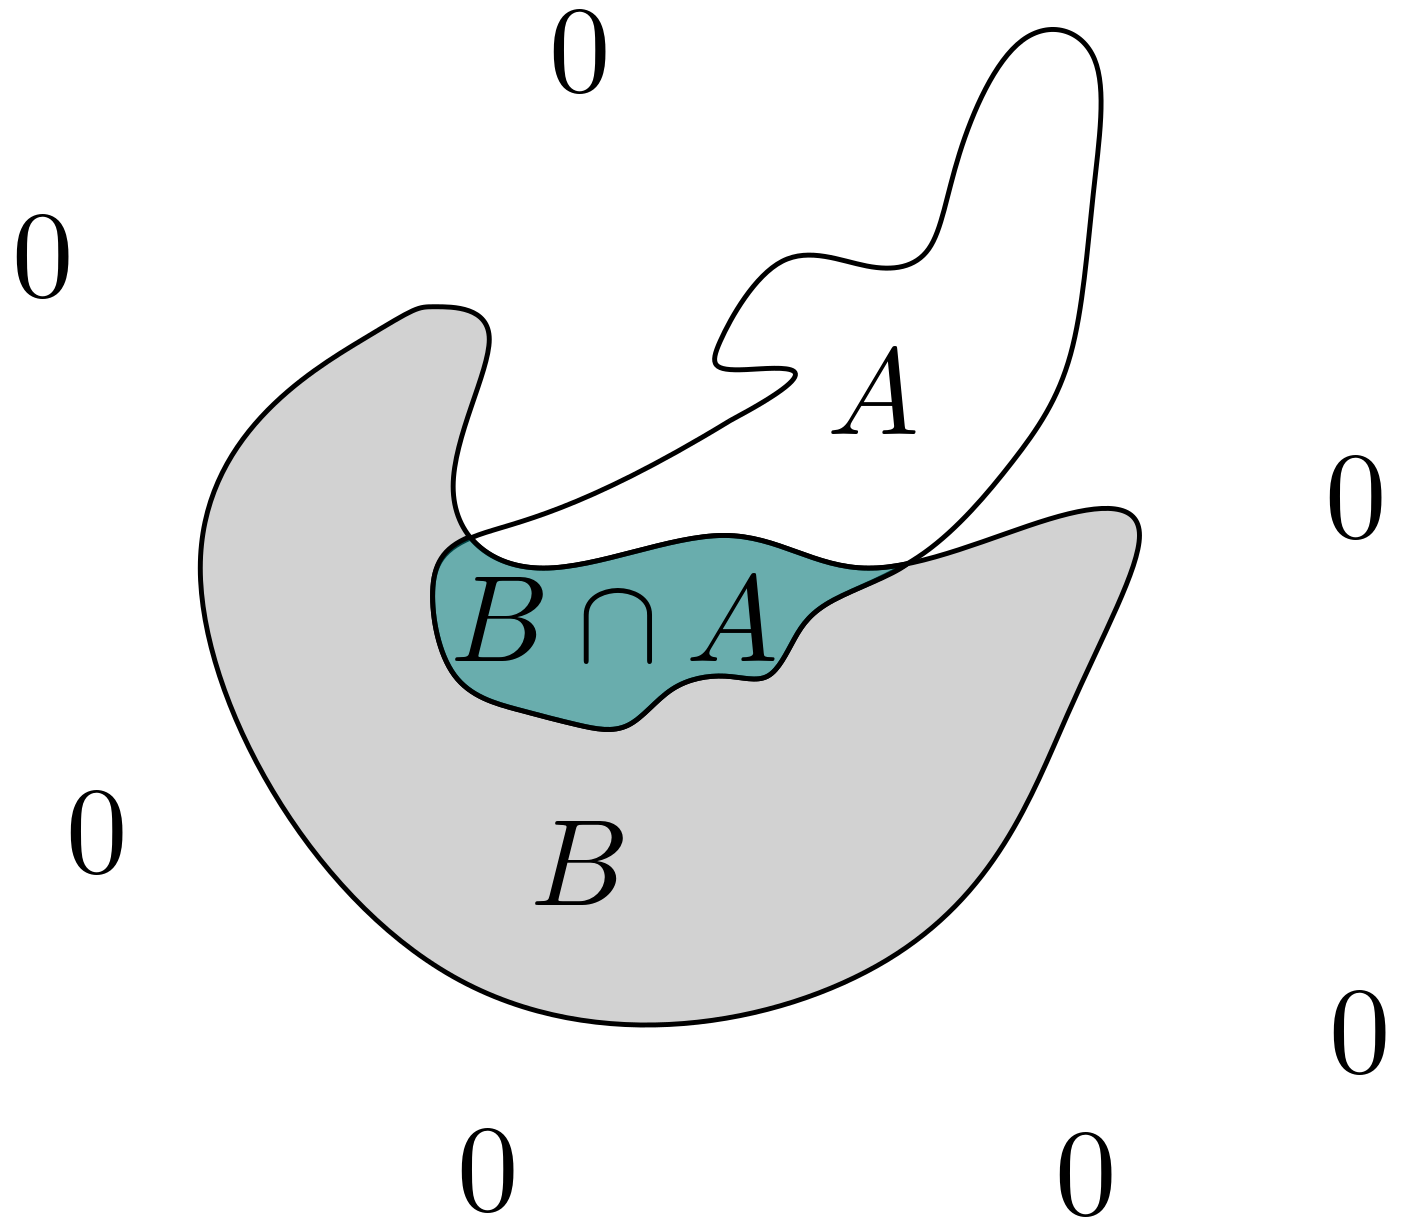
\includegraphics[width=0.25\textwidth]{MA4L14_1.png}
			\caption{Продолжение меры $H^\alpha$ нулем вне множества $B$.}
			\label{14_1}
		\end{figure}
		Таким образом, мы продолжили меру нулем вне множества $B$. Мера $\mu$ это конечная, $\sigma$-аддитивная мера на $\MB(\MR^n)$, тогда: $\forall m, \, \exists \, F_m$ - замкнутое множество: $F_m \subset B$ и верно: $\mu(B \setminus F_m) < \tfrac{1}{m}$ по теореме о приближении борелевскими. Тогда: 
		$$
 			B = \bigcup\limits_m F_m \cup B_0^F
		$$
		где $B_0^F$ это множество меры нуль. Заметим, что: $\mu(B \setminus F_m) = H^\alpha(B \setminus F_m)$, поскольку $\forall m, \, B \setminus F_m \subset B$. Для получения компактов можно взять кубы: $\MI_N = [-N, N]^n$ и представить $F_m$ в виде:
		$$
			F_m = \bigcup\limits_{N = 1}^{\infty}F_m \cap \MI_N
		$$
		где $F_m \cap \MI_N$ уже будут компактами;
		\item По предыдущему пункту: $E = \cup_j K_j \cup A$, где $A$ это множество $H^\alpha$-меры нуль. Тогда мы знаем, что: $f(E) = \cup_j f(K_j)\cup f(A)$, где $f(K_j)$ это компакты, а $f(A)$ это множество $H^\alpha$-меры нуль. Все эти множества измеримы $\Rightarrow$ мы получили измеримое множество. Из липшицевости будет верно:
		$$
			H^\alpha(f(E)) \leq \Lambda^\alpha{\cdot}H^\alpha(E) < \infty
		$$
	\end{enumerate}
\end{proof}
\begin{rem}
	Заметим также, что $F_m$ - замкнуты относительно $\MR^n$.
\end{rem}
\begin{rem}
	Заметим, что в пункте $2)$ $H^\alpha$ не является конечной мерой на борелевской $\sigma$-алгебре, даже если мы ограничим её на какой-либо куб. Если $\alpha$ будет малым, то мера будет бесконечной у многих множеств и применить теорему о приближении мы не сможем (там существенно было, что мера конечная). Заменить $\MR^n$ на борелевское множество мы также не можем, поскольку тогда поменяется топология: замкнутое множество в $B$ не тоже самое, что и замкнутое множество в $\MR^n$. Следовательно, правильным действием являлось продолжение $H^\alpha$ нулём вне $B$, получаем $\sigma$-аддитивную меру на всей борелевской $\sigma$-алгебре и применение к ней обычную теоремы о приближении.
\end{rem}

\subsection*{Связь меры $H^n$ и $\lambda$ на $\MR^n$}
\begin{prop}
	Пусть $n = 1$, тогда: $\forall E, \, H^1(E) = H_\delta^1(E) = \lambda(E)$ на $\MR$.
\end{prop}
\begin{proof}
	Пусть $\delta > 0$, по определению:
	$$
		H_\delta^1(E) = \inf\left\{\ddsum{j}{}\diam{F_j} \colon E \subset \cup_j F_j, \, \diam{F_j} \leq \delta\right\}, \quad
		\lambda(E) = \inf\left\{\ddsum{j}{}|\MI_j| \colon E \subset \cup_j \MI_j\right\}
	$$
	где $\MI_j$ это отрезки, $F_j$ это замкнутые множества на $\MR$ (отрезки) и верно, что $|\MI_j| = \diam{\MI_j}$. Поскольку отрезки всегда можно разбить на более мелкие, то можно считать, что: $\diam{\MI_j}\leq \delta$. Тем не менее, для меры Хаусдорфа используются произвольные замкнутые множества, следовательно: $H_\delta^1(E) \leq \lambda(E)$. Возьмем $F_j$ с диаметром $d_j = \diam{F_j}$ и возьмем отрезок: $\MI_j = [\inf{F_j}, \sup{F_j}]$, тогда: 
	$$
		|\MI_j| = d_j, \, F_j \subset \MI_j \Rightarrow \ddsum{j}{}\diam{F_j} = \ddsum{j}{}|\MI_j| \wedge E \subset \cup_j \MI_j
	$$
	Заметим, что $\sum_j |\MI_j| \geq \lambda(E)$, поскольку $\lambda(E)$ это точная нижняя грань таких сумм, тогда:
	$$
		\ddsum{j}{}\diam{F_j} \geq \lambda(E) \Rightarrow H_\delta^1(E) \geq \lambda(E) \Rightarrow H_\delta^1(E) = \lambda(E)
	$$
\end{proof}
\begin{rem}
	При $n = 1$ в определении $H_\delta^\alpha$ замкнутые множества можно заменить отрезками или интервалами. Замена интервалами возможна по тем же самым причинам по которым в мере Лебега можно было заменить отрезки интервалами: слегка увеличить и заменить отрезок интервалом, если получилось покрыть интервалами, то замена интервала на отрезок не меняет его диаметр (длину). В многомерном случае это уже не так и нельзя заменить множество шаром.
\end{rem}
\begin{exrc}
	Привести пример замкнутого множества $F$ на $\MR^2$ с $\diam{F} = r > 0$ такого, что не существует замкнутого шара: $\MB(a,\tfrac{r}{2}) \colon F \subset \MB(a,\tfrac{r}{2})$.
\end{exrc}

Рассмотрим теперь, что будет при $n > 1$.
\begin{theorem}
	Верны следующие утверждения:
	\begin{enumerate}[label = \arabic*)]
		\item $H^n(E) = 0 \Leftrightarrow \lambda(E) = 0$;
		\item $0< H^n([0,1]^n) < \infty$;
		\item $\MA_{H^n} = \MA_\lambda$ и $\exists \, c_n \in \MR, \, c_n > 0 \colon c_n H^n = \lambda$ на измеримых множествах;
	\end{enumerate}
\end{theorem}
\begin{proof}\hfill
	\begin{enumerate}[label=\arabic*)]
		\item $(\Leftarrow)$ Покажем, что $\lambda(E) = 0 \Rightarrow H^n(E) = 0$, для этого достаточно показать: $\forall \delta > 0,\, H_\delta^n(E) = 0$. Тогда:
		$$
			\lambda(E) = 0 \Rightarrow \forall \VE > 0, \, E \subset \cup_j \MI_j, \, \MI_j \text{ - замкнутые}, \, \ddsum{j}{}|\MI_j| < \VE
		$$
		Мы знаем, что можно считать $\MI_j$ кубами и $\diam{\MI_j} < \delta$. Пусть мы взяли куб $\MI_j$ с ребром $l_j$, тогда: 
		$$
			\diam{\MI_j} = \sqrt{n}{\cdot}l_j, \, |\MI_j| = l_j^n \Rightarrow(\diam{\MI_j})^n = n^{\tfrac{n}{2}}{\cdot}l_j^n = n^{\tfrac{n}{2}}{\cdot}|\MI_j| \Rightarrow 
		$$
		$$	
			\Rightarrow \ddsum{j}{}(\diam{\MI_j})^n = n^{\tfrac{n}{2}}{\cdot}\ddsum{j}{}|\MI_j| < n^{\tfrac{n}{2}}{\cdot}\VE \Rightarrow H_\delta^n(E) \leq n^{\tfrac{n}{2}}{\cdot}\VE \xrightarrow[\VE \to 0]{} 0 \Rightarrow H_\delta^n(E) = 0
		$$
		$(\Rightarrow)$ Пусть теперь $H^n(E) = 0$, тогда $\forall \delta > 0, \, H_\delta^n(E) = 0$. Зафиксируем $\delta = 1$, тогда:
		$$
			\forall \VE > 0, \, E \subset \bigcup\limits_j F_j,\, F_j \text{ - замкнутые}, \, \diam{F_j} < 1, \, \ddsum{j}{}(\diam{F_j})^n < \VE
		$$
		Если $d_j = \diam{F_j}$ и $a_j \in F_j$, то верно: 
		$$
			F_j \subset \ovl{\MB}(a_j,d_j) \Rightarrow \lambda(\ovl{\MB}(a_j,d_j)) = \omega_n{\cdot}d_j^n
		$$ 
		где $\omega_n$ это некоторая константа (объем единичного шара). При этом мы получаем:
		$$
			E \subset \bigcup\limits_j \ovl{\MB}(a_j, d_j) \Rightarrow \lambda(E) \leq \ddsum{j}{}\lambda(\ovl{\MB}(a_j, d_j)) =  \omega_n{\cdot}\ddsum{j}{}(\diam{F_j})^n < \omega_n{\cdot}\VE \xrightarrow[\VE \to 0]{} 0 \Rightarrow \lambda(E) = 0
		$$
		\item Очевидно, что $H^n([0,1]^n) > 0$, так как $\lambda([0,1]^n) = 1 > 0$. Пусть $\delta > 0$, хотим получить какую-то оценку $H^n([0,1]^n)$. Разобьем куб $[0,1]^n$ на более мелкие кубы $K_j$ с рёбрами $\tfrac{1}{N}$, тогда: 
		$$
			\diam{K_j} = \dfrac{\sqrt{n}}{N} \Rightarrow \exists\, N \colon \diam{K_j} \leq \delta \Rightarrow \ddsum{j}{}(\diam{K_j})^n = n^{\tfrac{n}{2}}{\cdot}\ddsum{j}{}\dfrac{1}{N^n} = n^{\tfrac{n}{2}}{\cdot}1 = n^{\tfrac{n}{2}}
		$$
		где сумма равна $1$ так как из $K_j$ у нас составлен большой куб, тогда: 
		$$
			H_\delta^n([0,1]^n) \leq n^{\tfrac{n}{2}}
		$$ 
		Поскольку у нас $n$ фиксирована, то при $\delta \to 0$ будет верно:
		$$
			H^n([0,1]^n) \leq n^{\tfrac{n}{2}} < \infty
		$$
		\item Мы знаем, что верно соотношение: 
		$$
			E \in \MA_\lambda \Leftrightarrow E = B \cup B_0^\lambda
		$$ 
		где $B$ это борелевское и $B_0^\lambda$ множество меры $\lambda$ нуль. Аналогично, известно, что: 
		$$
			E \in \MA_{H^n} \Rightarrow E = \bigcup\limits_N E \cap [-N,N]^n
		$$ 
		где $E \cap [-N,N]^n$ это множество конечной меры $H^n$, поскольку единичный куб имеет конечную меру, а этот куб отличается от единичного гомотетией, которая есть липшицево отображение $\Rightarrow$ образ множества конечной меры является множеством конечной меры $\Rightarrow E \cap [-N,N]^n = B_N \cup A_N$, где $B_N$ - борелевское, а $A_N$ - множество меры нуль $H^n$. Тогда: 
		$$
			E = \bigcup\limits_N B_N \cup \bigcup\limits_N A_N
		$$ 
		то есть $E$ это объединение борелевских множеств и счетного числа множеств меры нуль - множества меры нуль по $H^n$ и по $\lambda$ (поскольку мы знаем, что это одно и то же). А если оно представляется в таком виде, то оно конечно измеримо по $H^n$ (борелевские измеримы и множество меры нуль измеримы). Следовательно, $\MA_\lambda = \MA_{H^n}$.
		
		Заметим, что $H^n([0,1]^n) > 0 \Rightarrow$ можно умножить на константу так, чтобы получили $1$:
		$$
			\exists\, c_n \colon c_n{\cdot}H^n([0,1]^n) = 1 = \lambda([0,1]^n)
		$$ 
		Вычисление этой $c_n$ достаточно сложно, для этого нужно изодиаметрическое неравенство и мы его вычислять не будем. Докажем, что $c_n{\cdot}H^n = \lambda$ на измеримых множествах. Возьмем куб $[0,1]^n$ и поделим его сторону на $N$ частей $\Rightarrow$ весь куб разбивается на $N^n$ кубиков $K_j$, причем они конгруэнтны, то есть $K_i$ можно получить из $K_j$ движением. Следовательно: 
		$$
			H^n(K_i) = H^n(K_j), \, H^n(K_i \cap K_j) = 0
		$$ 
		где последнее верно поскольку либо $K_i \cap K_j = \VN$, либо $K_i \cap K_j$ это множество меры нуль. Тогда:
		$$
			1 = c_n{\cdot}H^n([0,1]^n) = 1 = \ddsum{j}{}c_nH^n(K_j) = N^n{\cdot}c_n{\cdot}H^n(K_1) \Rightarrow c_n{\cdot}H^n(K_j) = \dfrac{1}{N^n} = \lambda(K_j)
		$$
		Следовательно, $c_n{\cdot}H^n$ и $\lambda$ совпадают на кубах с ребром $\tfrac{M}{N} \in \MQ$, поскольку такой куб может быть составлен любым образом из кубиков $K_j$, а для этих кубиков меры совпадают $\Rightarrow c_n{\cdot}H^n$ и $\lambda$ совпадают на открытых множествах, поскольку любое открытое можно представить в виде объединения счетного числа кубиков, причем мы делали построение с шагом $\tfrac{1}{2^r}$, которые пересекаться могут лишь по границам (см. лекцию $5$). 
		\begin{figure}[H]
			\centering
			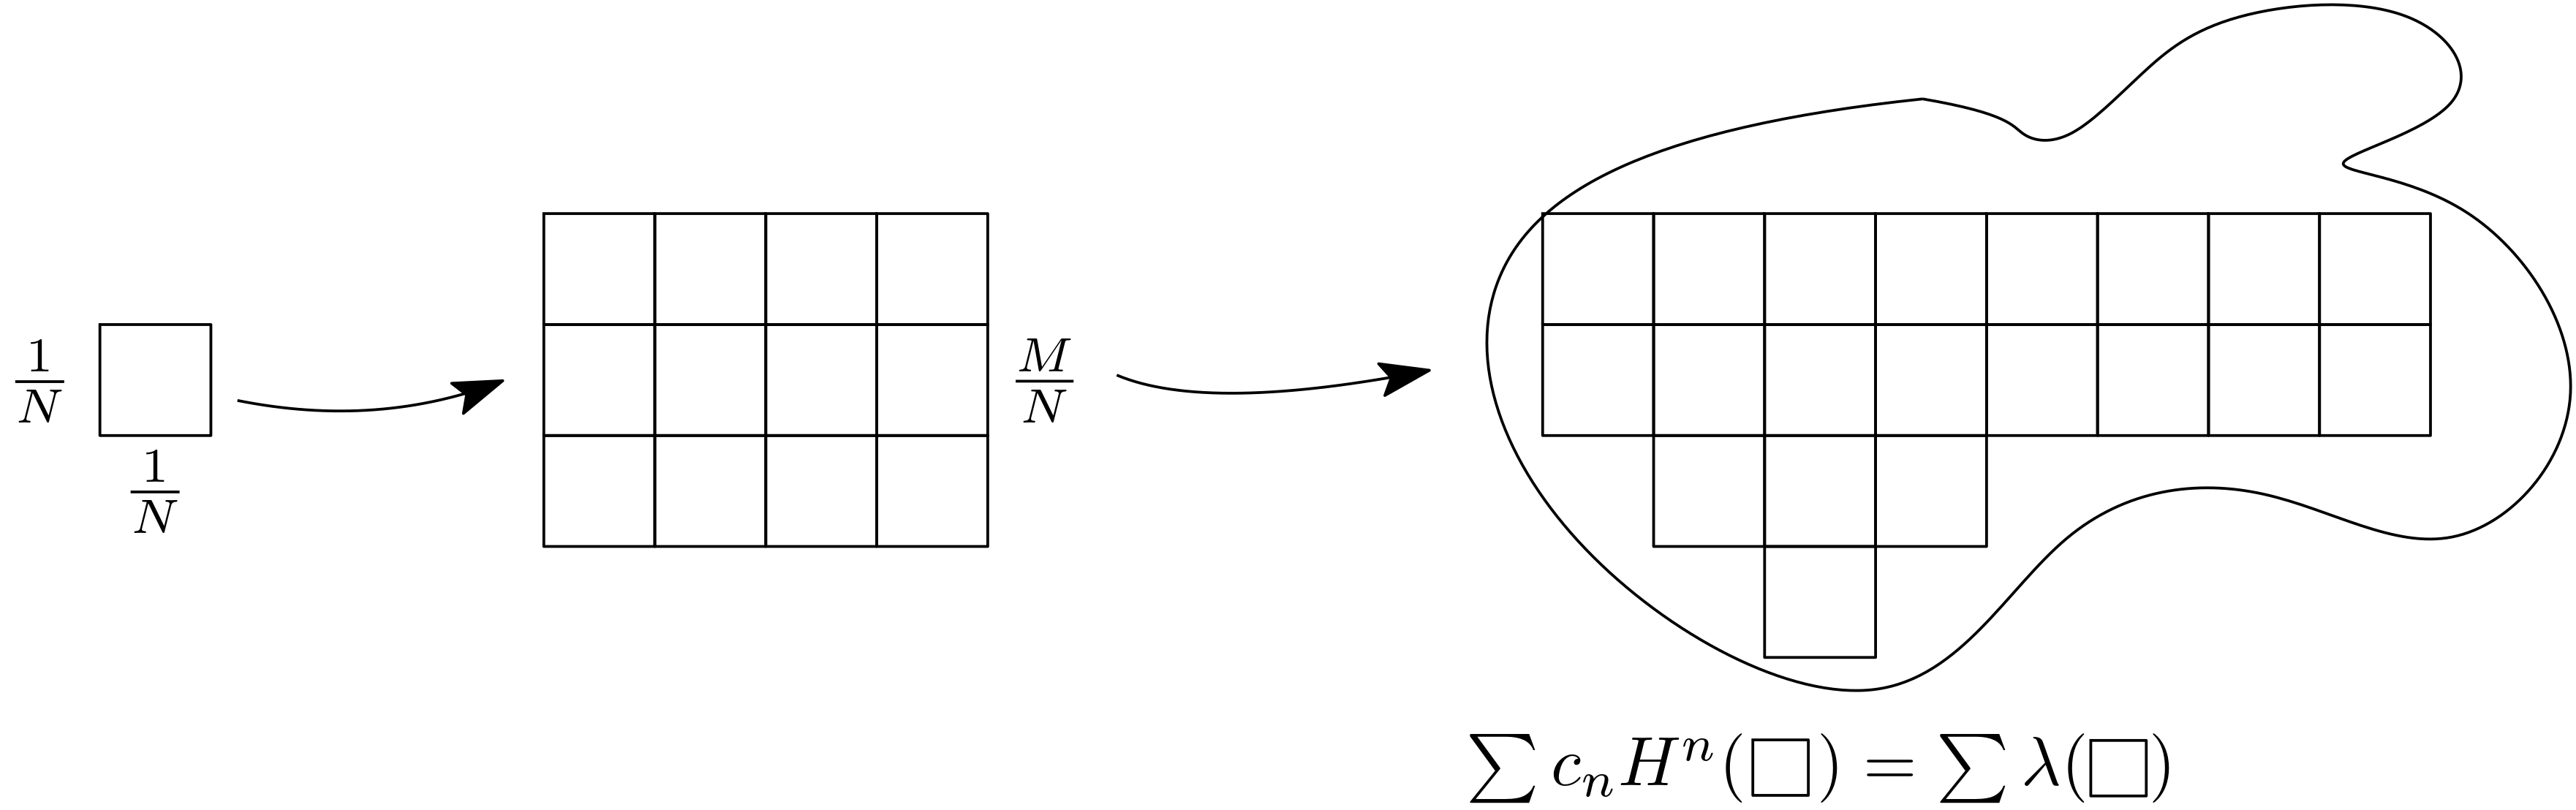
\includegraphics[width=0.75\textwidth]{MA4L14_2.png}
			\caption{Совпадение мер на открытых множествах, построением из кубиков с ребрами $\tfrac{M}{N} \in \MQ$.}
			\label{14_2}
		\end{figure}
		Меры совпадают на открытых множествах $\Rightarrow$ можем брать открытые множества из куба $[-N,N]^n$ и применять теорему о совпадении двух мер $\Rightarrow c_n{\cdot}H^n$ и $\lambda$ - конечные меры на $\MB([-N,N]^n)$ и совпадают на открытых множествах, а поскольку $[-N,N]$ можно брать любое, то $c_n{\cdot}H^n$ и $\lambda$ совпадают на всех $\MB(\MR^n) \Rightarrow$ так как любое измеримое множество это борелевское плюс множество меры нуль, то $c_n{\cdot}H^n$ и $\lambda$ совпадают на измеримых множествах;
	\end{enumerate}
\end{proof}
Далее, всегда считаем, что $H^\alpha$ умножается на $c_\alpha$ так, что $H^k$ на $\MR^k$ совпадает с $\lambda$.

\begin{corollary}
	Пусть $\Pi_k$ - $k$-мерная, аффинная плоскость в $\MR^n$ и $\lambda_{\Pi_k}$ - мера Лебега на $\Pi_k$, тогда $H^k$ на $\Pi_k$ совпадает с $\lambda_{\Pi_k}$. В частности, если $\Pi_k = L(\MR^k), \, L(x) = Ax + b, \, \rk{A} = k$, то:
	$$
		H^k(L(E)) = \sqrt{\det{(A^TA)}}\lambda(E)
	$$ 
	для всякого измеримого $E$ в $\MR^k$.
\end{corollary}
\begin{proof}
	Очевидно, поскольку мера Хаусдорфа, построенная на замкнутом подмножестве (а $\Pi_k$ это замкнутое подмножество), совпадает с мерой Лебега. А если мы считаем, что работаем только в плоскости $\Pi_k$, то дальше ситуация неотличима от $\MR^k$: ввели на $\Pi_k$ ортогональную систему координат, плоскость отождествилась с $\MR^k$, а мера Хаусдорфа совпала с мерой Лебега.
\end{proof}
Можно считать, что $H^k$ это мера Хаусдорфа построенная внутри этой $k$-мерной плоскости $\Pi_k$, при построении меры Хаусдорфа система координат не используется (используется только метрика - диаметр считается), мера Лебега не зависит от системы координат $\Rightarrow$ выбираем систему координат $\Rightarrow$ получаем меру Хаусдорфа в $\MR^k$ и меру Лебега в $\MR^k$, выше мы доказали, что они совпадают. 
\begin{rem}
	Мера Хаусдорфа не зависит от системы координат по построению, используется только метрика (считается диаметр), то есть она инвариантна относительно прямоугольной системы координат (чтобы расстояния сохранялись).
\end{rem}

\end{document}